\documentclass{standalone}
\usepackage{tikz}
\usepackage{pgfplots}
\pgfplotsset{width=32cm,height=18cm,compat=1.3}
\pgfplotsset{every tick label/.append style={font=\Huge}}
\usepackage{filecontents}

\usetikzlibrary{patterns}

\definecolor{citrine}{rgb}{0.89, 0.82, 0.04}

\begin{document}
	\centering
		\vspace{1.5em}
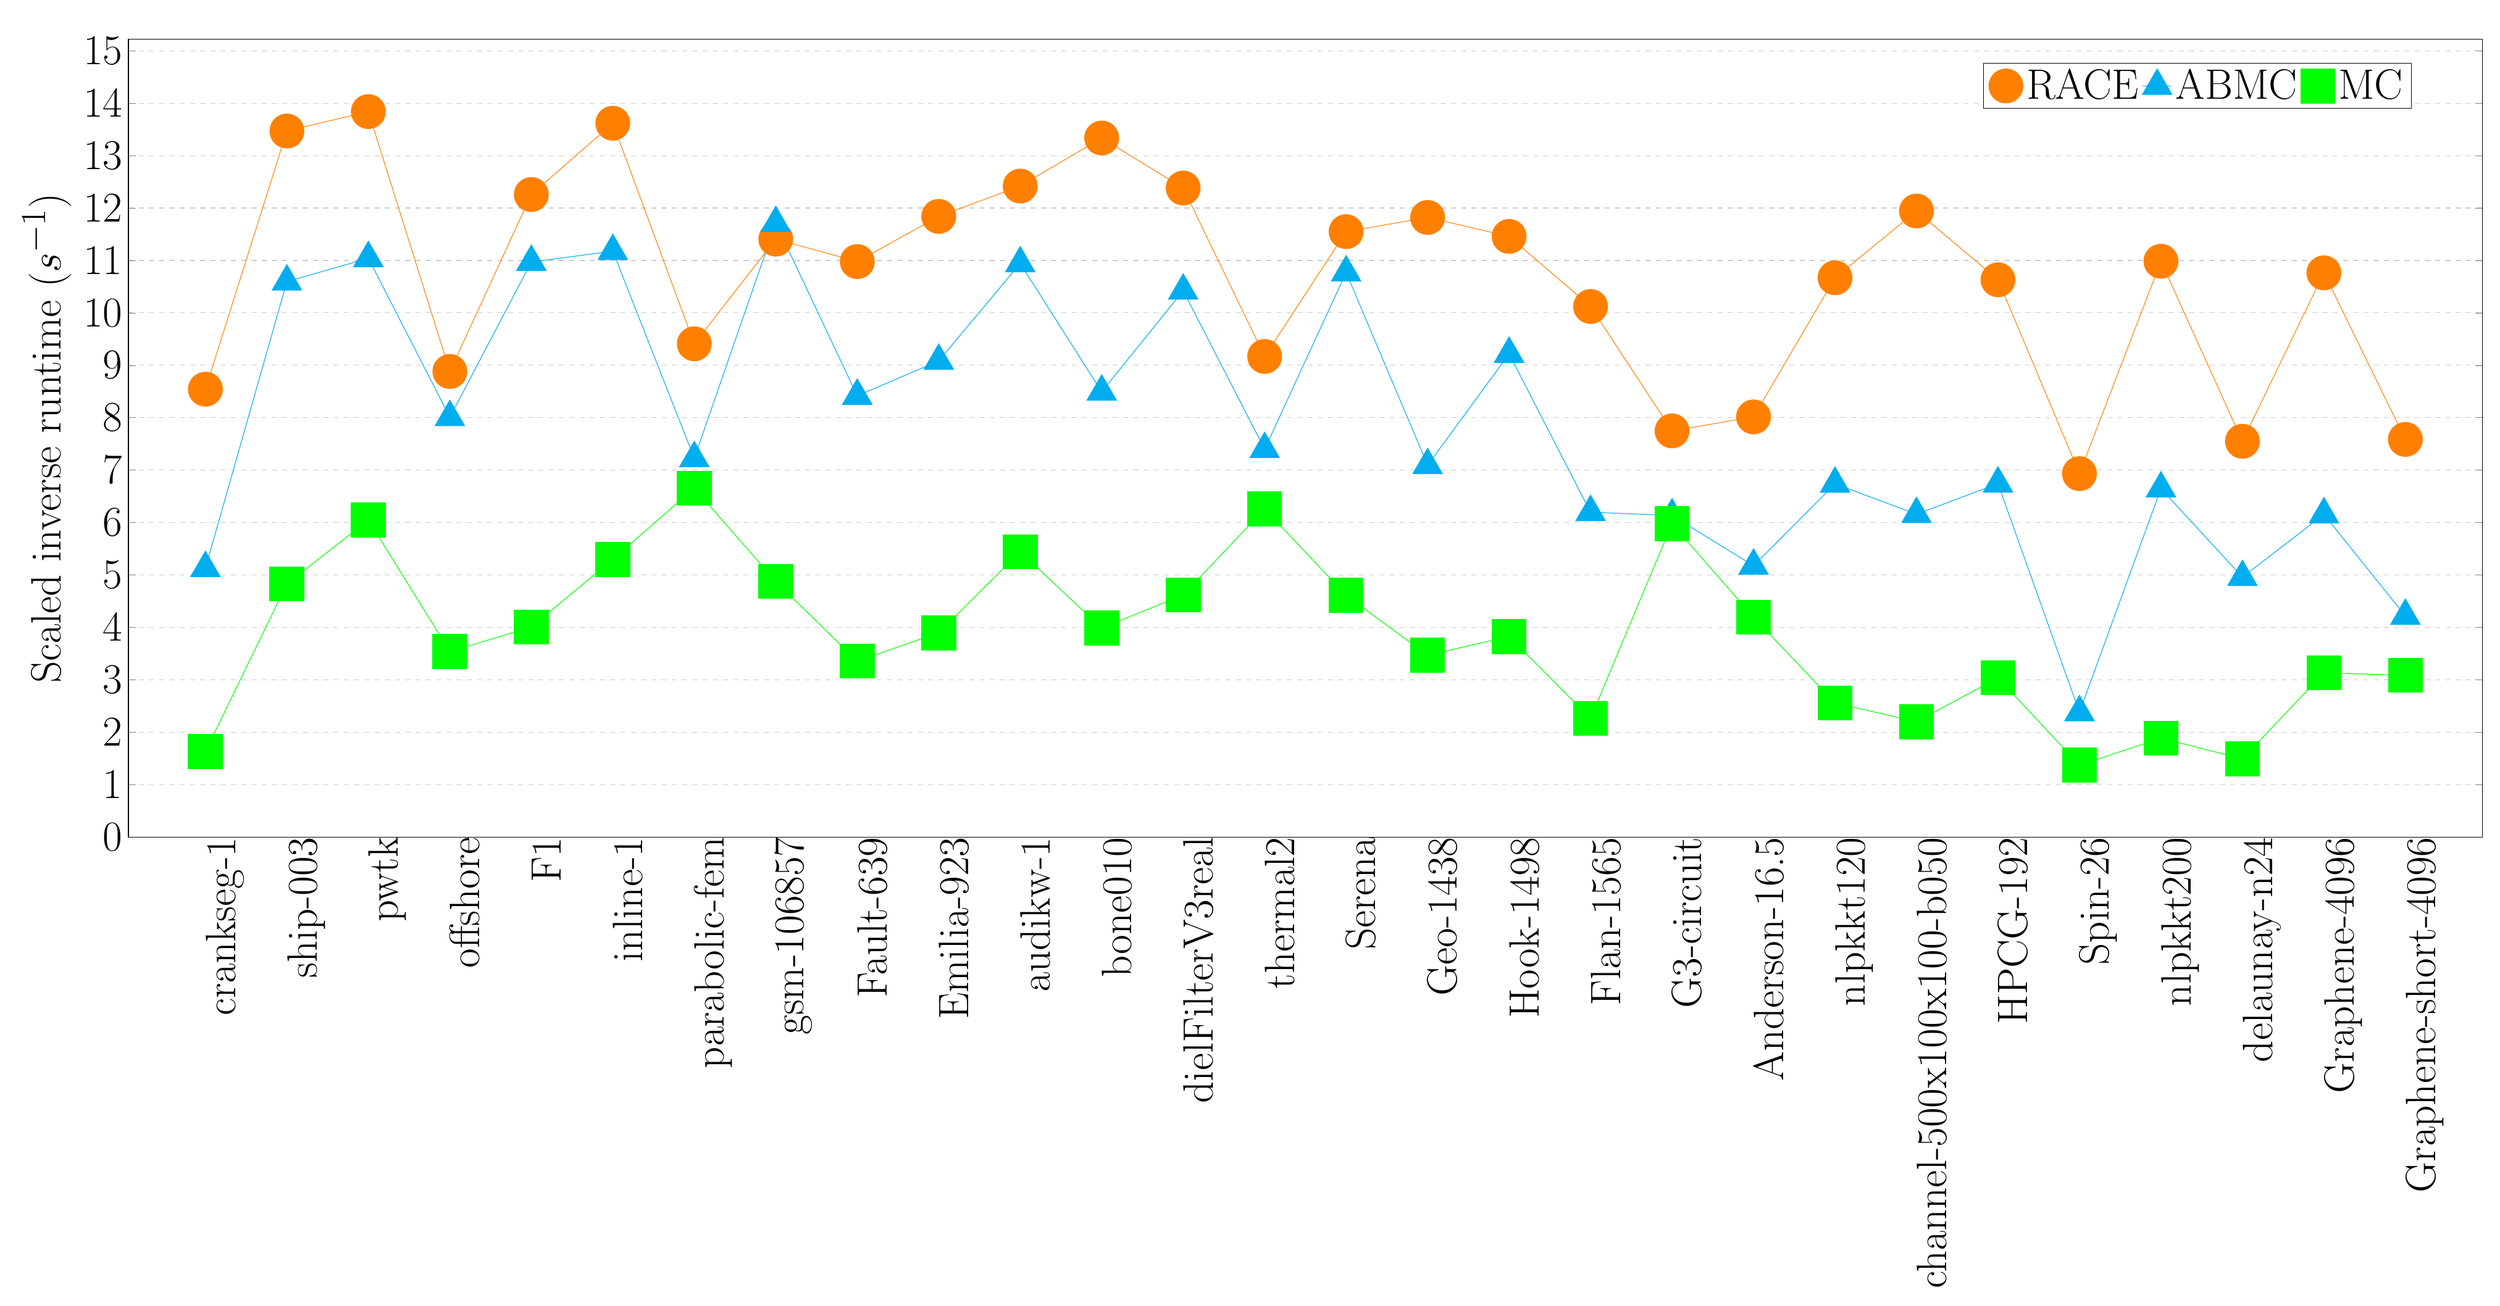
\begin{tikzpicture}
		%	\node at (13.25,15) {\LARGE{}};
			\begin{axis}[
		%	xmin=0.25, xmax=7.25,
			ymin=0, %ymax=3.25,
			xtick={1, 2, 3, 4, 5, 6, 7, 8, 9, 10, 11, 12, 13, 14, 15, 16, 17, 18, 19, 20, 21, 22, 23, 24, 25, 26, 27, 28},
		%	ytick={0,0.5,1,1.5,2,2.5,3},
			xticklabels={crankseg-1, ship-003, pwtk, offshore, F1, inline-1, parabolic-fem, gsm-106857, Fault-639, Emilia-923, audikw-1, bone010, dielFilterV3real, thermal2, Serena, Geo-1438, Hook-1498, Flan-1565, G3-circuit, Anderson-16.5, nlpkkt120, channel-500x100x100-b050, HPCG-192, Spin-26, nlpkkt200, delaunay-n24, Graphene-4096, Graphene-short-4096},
			width  = 50cm,
			height = 18cm,
			major x tick style = transparent,
			%	minor ytick={1, 5, 10, 15, 20, 25, 30 ,35,40},
			grid = minor,	
			%add_bar_commands
			ymajorgrids = true,
			grid style={dashed, gray!40},
			ylabel = {\Huge{Scaled inverse runtime ($s^{-1}$)}},
		%	symbolic x coords={Graphene-2048-2048, Graphene-4096-4096, Spin-24-24-24},
			x tick label style={rotate=90, anchor=north east, inner sep=0mm, font={\Huge}},
			tick label style={font={\Huge}},
			scaled y ticks = false,
			enlarge x limits=0.035,
			legend cell align=left,
			legend style={font=\Huge},
			legend columns=-1,
			legend style={
				%at={(1,1.05)},
				%anchor=south east,
				%column sep=1ex,
				legend pos=north east
			},
			%spl_legend_code
			title= {\Huge\scalebox{1.5}{{}}}
			]

\addplot[ mark=*, mark size=10pt, mark options={orange}, draw=orange , y filter/.code={\pgfmathparse{\pgfmathresult*1000}\pgfmathresult}] plot coordinates{(1,.00854272307692307692) (2,.01346882254901960784) (3,.01383979509803921568) (4,.00888176990291262135) (5,.01225669108910891089) (6,.01361732500000000000) (7,.00940900194174757281) (8,.01140629100000000000) (9,.01097814128440366972) (10,.01184031495327102803) (11,.01241869900990099009) (12,.01333580099009900990) (13,.01238193564356435643) (14,.00916779603960396039) (15,.01154918383838383838) (16,.01182014313725490196) (17,.01145815242718446601) (18,.01012141278195488721) (19,.00774722427184466019) (20,.00801449819819819819) (21,.01066906435643564356) (22,.01194286764705882352) (23,.01063077272727272727) (24,.00693199274193548387) (25,.01098451666666666666) (26,.00754907156862745098) (27,.01076298118811881188) (28,.00758556831683168316)};
\addplot[ mark=triangle*, mark size=10pt, mark options={cyan}, draw=cyan , y filter/.code={\pgfmathparse{\pgfmathresult*1000}\pgfmathresult}] plot coordinates{(1,.00512872941176470588) (2,.01059520909090909090) (3,.01104178770491803278) (4,.00800800098039215686) (5,.01096985277777777777) (6,.01117693853211009174) (7,.00722462000000000000) (8,.01171085049504950495) (9,.00841625890410958904) (10,.00908392109375000000) (11,.01094233679245283018) (12,.00849387857142857142) (13,.01042162857142857142) (14,.00739910761904761904) (15,.01076890500000000000) (16,.00709226666666666666) (17,.00921667606837606837) (18,.00619610211640211640) (19,.00613335294117647058) (20,.00517406071428571428) (21,.00673643032786885245) (22,.00615895737704918032) (23,.00674099349593495934) (24,.00237763333333333333) (25,.00664720964912280701) (26,.00495737586206896551) (27,.00615319851851851851) (28,.00421802192982456140)};
\addplot[ mark=square*, mark size=10pt, mark options={green}, draw=green , y filter/.code={\pgfmathparse{\pgfmathresult*1000}\pgfmathresult}] plot coordinates{(1,.00163132440944881889) (2,.00482913716814159292) (3,.00604677024793388429) (4,.00353736166666666666) (5,.00400742480000000000) (6,.00529540990099009900) (7,.00665603566433566433) (8,.00487397272727272727) (9,.00335574907975460122) (10,.00389533469387755102) (11,.00544275252525252525) (12,.00398660740740740740) (13,.00461716746031746031) (14,.00625954338235294117) (15,.00460889823008849557) (16,.00346840566037735849) (17,.00382457464788732394) (18,.00226408260869565217) (19,.00597724462809917355) (20,.00419089007633587786) (21,.00255797727272727272) (22,.00219792661870503597) (23,.00303785147058823529) (24,.00137003333333333333) (25,.00188547014925373134) (26,.00149133164556962025) (27,.00313092965517241379) (28,.00308532352941176470)};
	%addplot cmd

	\legend{RACE, ABMC, MC}

	\end{axis}			
\end{tikzpicture}

\end{document}

